\section{Control module}

The control module is responsible for coordinating the activity of the
other parts of the image processor and for data transfer within the
image processor. A visual overview of the control module is given in
figure \ref{fig:control-module}.

\begin{figure}[h!]
\centering
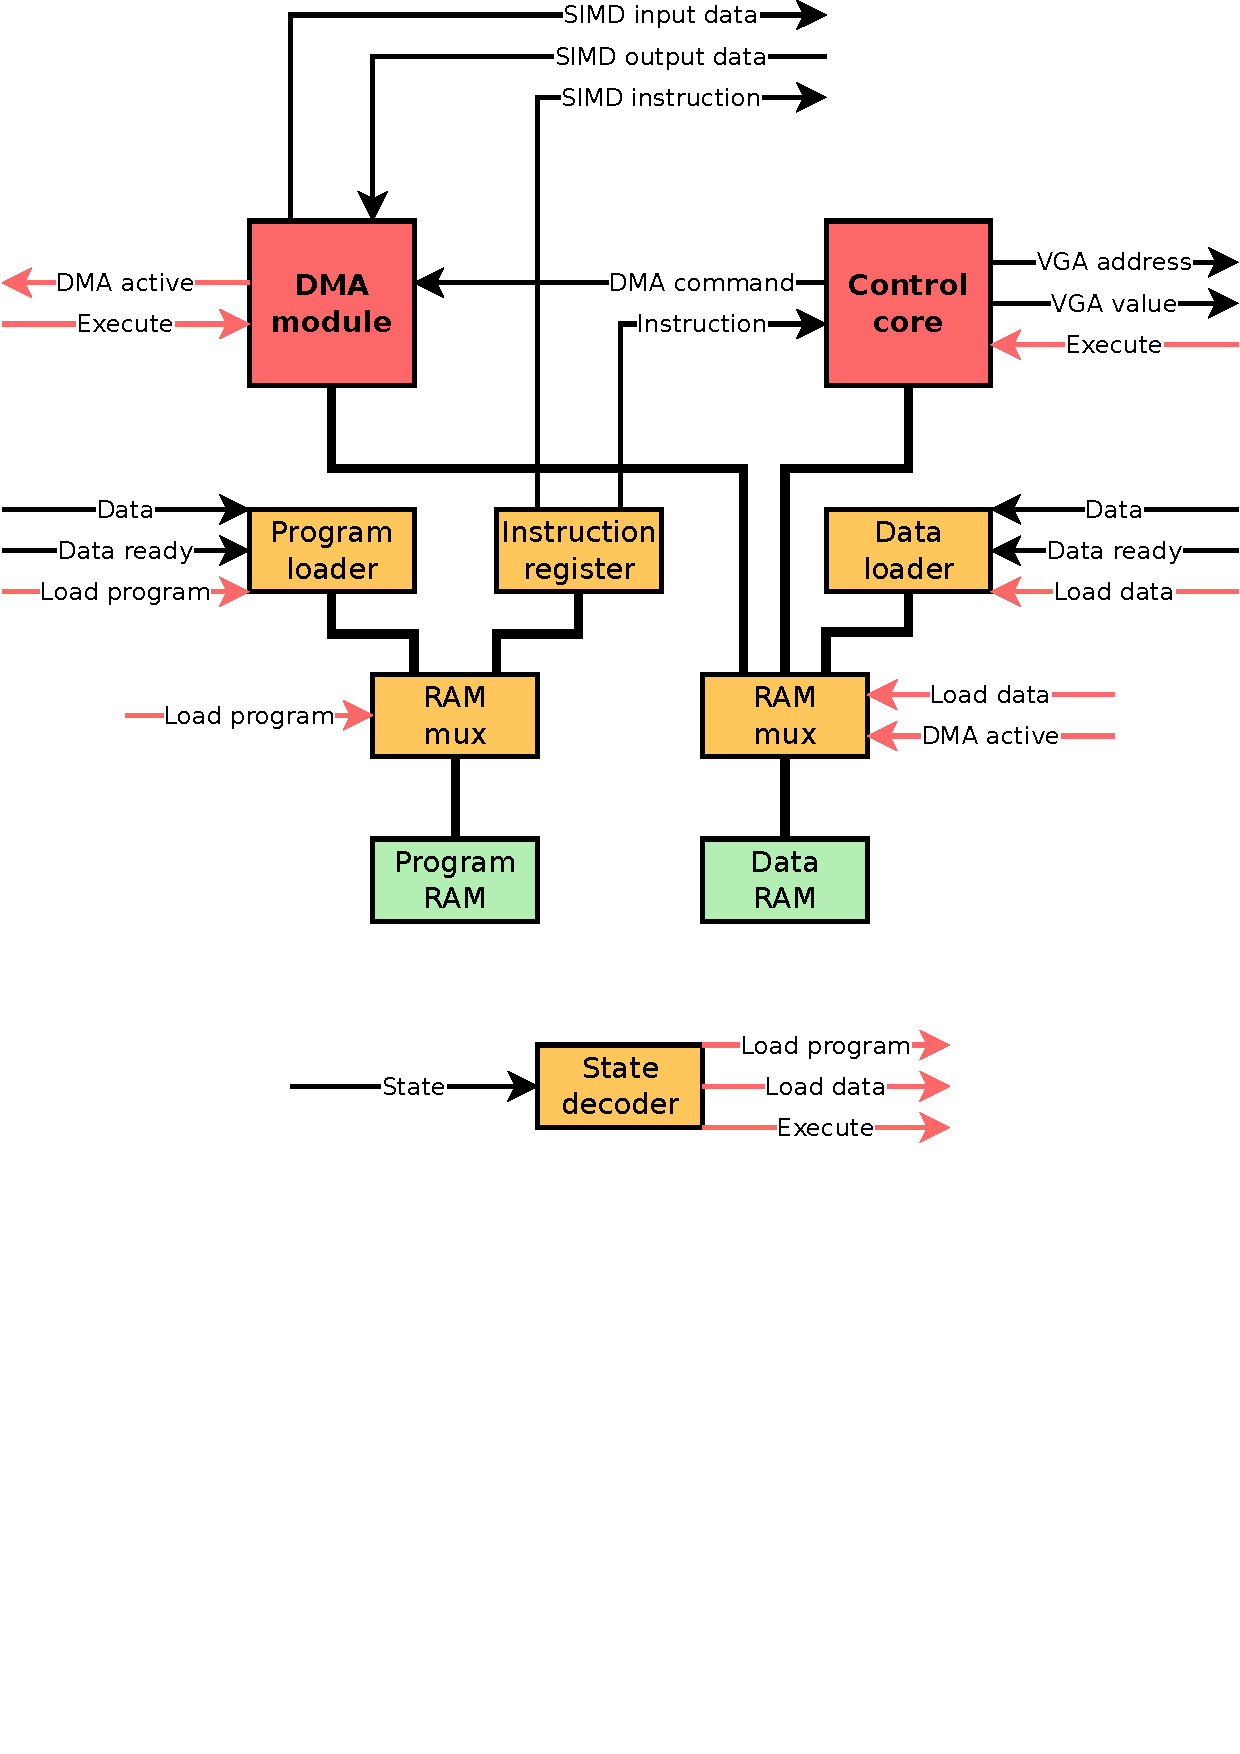
\includegraphics[width=\linewidth,clip,trim=0 10cm 0 0]
                {fig/fpga/control_module.pdf}
\caption[Control module]
        {An overview of the control module of the image processor.}
\label{fig:control-module}
\end{figure}


The control module decodes the state signal set by the AVR, and enables,
disables and resets components accordingly. It is also responsible for
performing data transfer between the AVR and the program/data RAM.

The control module contains the CPU core that is used for non-SIMD
instructions during program execution. This CPU core, henceforth
referred to as the \emph{control core}, is mainly concerned with keeping
track of which parts of the data set the SIMD array is currently
processing.

